\PassOptionsToPackage{dvipsnames}{xcolor}
\documentclass[hyperref={pdfpagelabels=false}]{beamer}
% beamer already loads hyperref; do NOT load \usepackage{hyperref} again.

\usepackage{ragged2e} % 文字向兩邊對齊
\renewcommand{\raggedright}{\leftskip=0pt \rightskip=0pt plus 0cm}

\usepackage{listings}
\usepackage{lmodern}
\usepackage{fontspec}
\usepackage{xeCJK}
\setCJKmainfont{Noto Sans CJK TC}
%（可選）若你會用到無襯線中文或等寬中文，建議補上：
\setCJKsansfont{Noto Sans CJK TC}
\setCJKmonofont{Noto Sans Mono CJK TC}

\usepackage[english]{babel}
\usepackage{amsmath,amssymb,amsfonts,amsthm}

% hyperref settings (since beamer already loads hyperref)
\hypersetup{
  colorlinks=true,
  urlcolor=blue,
  citecolor=blue,
  pdfborder={0 0 0}
}

\usepackage{accsupp}% http://ctan.org/pkg/accsupp
\newcommand{\emptyaccsupp}[1]{\BeginAccSupp{ActualText={}}#1\EndAccSupp{}}

\usepackage{tikz}
\usetikzlibrary{arrows,arrows.meta,decorations.pathmorphing,backgrounds,fit,positioning,shapes.symbols,chains}

\usepackage{booktabs}
\usepackage{threeparttable}
\usepackage{colortbl}
\usepackage{comment} 
\usepackage{xcolor}
\usetikzlibrary{tikzmark}

\newcommand{\indep}{\perp\!\!\!\perp}
\newcommand{\nindep}{\not\!\perp\!\!\!\perp}
\newcommand{\E}{\mathrm{E}}
\newcommand{\Var}{\mathrm{Var}}

\beamertemplatefootpagenumber


%%%%%%%%%%%%%%%%%%%%%%%%%%%%%%%%%%%%%%%%%%%%%%%%%%%%%%%%%%%%%%%%%%%%%%%%%%%%%%
% LaTeX snippet: language and style definition of Stata for listings package.
%                [listings](http://www.ctan.org/pkg/listings) 
%                [Stata](http://www.stata.com/)
%
% Usage:
%     Copy the code into your preamble, or import it by `\include` .
%     then in your doc:
%     \lstinputlisting[style=numbers]{DO-SCRIPT}
%     \lstinputlisting[style=numbers, style=stata-editor]{DO-SCRIPT}
%     \lstinputlisting[style=nonumbers, frame=none]{DO-SCRIPT}
% How it works:
%     - The language is defined by `\lstdefinelanguage{Stata}`
%     - Four styles is defined by `\lstdefinestyle{STYLE-NAME}`, 
%       they are: numbers and no numbers, plain(black and white) and colorful
%       (colored roughly like stata editor.)
% Tips:
%     - Generally you only need to set your default in the last part,
%       that is, code inside of `\lstset`.
%     - Add more keywords(I can not list all of them) in the `\lstset` part.
%     - Do NOT leave any blank lines in commands
%       (`\lstddefinelanguage', `\lstdefinestyle` and `\lstset`)
%
% update: 2014-04-16
% version: 0.1
% author: kongs
% licence: MIT
% url: https://gist.github.com/kongs-sublime/10862838
%
% TODO: 
%       - finish keyword list.
%       - precise colors that match stata editor?
%       - make it flexible(fonts and style)
%
%%%%%%%%%%%%%%%%%%%%%%%%%%%%%%%%%%%%%%%%%%%%%%%%%%%%%%%%%%%%%%%%%%%%%%%%%%%%%%


% langugae defination
\lstdefinelanguage{Stata}{
	% Left for users to add missing commands,
	% with possibility of choosing different style.
	morekeywords=,
	% Popular add-on commands
	morekeywords=[2]{cntrade, chinafin, 
		wbopendata, spmap,
	},
	% System commands
	morekeywords=[3]{regress, summarize, 
		display,
	},
	% Keywords
	morekeywords=[4]{forvalues, if, foreach, set},
	% Built-in functions
	morekeywords=[5]{rnormal, runiform},
	morecomment=[l]{//},
	% morecomment=[l]{*},  // `*` maybe used as multiply operator. So use `//` as line comment.
	morecomment=[s]{/*}{*/},
	% morecomment=[s]{,}{//},
	% The following is used by macros, like `lags'.
	morecomment=[n][keywordstyle9]{`}{'},
	morestring=[b]",
	sensitive=true,
}

\lstdefinestyle{numbers}{
	numbers=left, 
	stepnumber=1, 
	numberstyle=\tiny\emptyaccsupp,
	xleftmargin=2em,
}

\lstdefinestyle{nonumbers}{
	numbers=none,
}

\lstdefinestyle{stata-plain}{
	language=Stata,
	basicstyle=\scriptsize\ttfamily,
}

\lstdefinestyle{stata-editor}{
	language=Stata,
	basicstyle=\scriptsize\ttfamily,
	keywordstyle={\color{NavyBlue}},  
	keywordstyle=[2]{\color{NavyBlue}},
	keywordstyle=[3]{\color{NavyBlue}},
	keywordstyle=[4]{\color{NavyBlue}},
	keywordstyle=[5]{\color{Blue}},
	keywordstyle=[9]{\color{TealBlue}},
	stringstyle=\color{Maroon},
	commentstyle=\color{OliveGreen},
}
\lstdefinestyle{r-style}{
	language=R,
	basicstyle=\scriptsize\ttfamily,
	keywordstyle=\color{NavyBlue},
	commentstyle=\color{OliveGreen},
	stringstyle=\color{Maroon},
}


\lstset{
	language=Stata,
	style=stata-editor,
	style=numbers,
	showstringspaces=false,
	breaklines,
	frame=single,
	backgroundcolor=\color{gray!5},
	% To add missing commands
	% morekeywords={xtreg, xtunitroot},
}




\title[Causal Forest]{Causal Machine Learning (III): Causal Forest}
%\subtitle{v5 -- labor economics example}

%\subtitle
%{免除部分負擔對幼兒醫療利用與健康的影響:斷點迴歸分析}

%\author 
%{Tzu-Ting Yang\inst{1} \and Hsing-Wen Han\inst{2} \and Hsien-Ming Lien\inst{3}}

%\institute[short]{\inst{1} Academia Sinica \and \inst{2} Tamkang University \and \inst{3} National Chengchi University}




\author 
{Prof. Tzu-Ting Yang  \\ 楊子霆}

%\institute{Institute of Economics, Academia Sinica  \\ Econ, NTU}
\institute{Institute of Economics, Academia Sinica  \\ 中央研究院經濟研究所}
%\institute{Institute of Economics, Academia Sinica  \\ Econ, NTU}
%\institute{Institute of Economics, Academia Sinica  \\ IMES/IDAS, NTU}


%\author 
%{楊子霆 \\ 中研院經濟所}

%\institute 
%{中正大學國際經濟專題研討}




\date
{\today}

\usetheme{CambridgeUS}
%\usecolortheme{seahorse}
\setbeamertemplate{footline}{%
	\hfill\usebeamercolor[fg]{page number in head/foot}%
	\usebeamerfont{page number in head/foot}%
	\insertframenumber\,/\,\inserttotalframenumber\hspace{1em}\vspace{2pt}%
}

% \usetheme{Boadilla}
% %\useinnertheme{rectangles}

% %\usetheme{CambridgeUS}
% \usecolortheme{seahorse}
% \setbeamertemplate{footline}{%
% 	\hfill\usebeamercolor[fg]{page number in head/foot}%
% 	\usebeamerfont{page number in head/foot}%
% 	\insertframenumber\,/\,\inserttotalframenumber\hspace{1em}\vspace{2pt}%
% }


% \usepackage{beamerthemeshadow}
% %\usecolortheme{seahorse}
% \setbeamertemplate{footline}{%
% 	\hfill\usebeamercolor[fg]{page number in head/foot}%
% 	\usebeamerfont{page number in head/foot}%
% 	\insertframenumber\,/\,\inserttotalframenumber\hspace{1em}\vspace{2pt}%
% }


%\usepackage{beamerthemeshadow}

\beamersetuncovermixins{\opaqueness<1>{25}}{\opaqueness<2->{15}}

\begin{document}

\begin{frame}
  \titlepage
\end{frame}

%=============================================================
\title[]
{Main Idea}

\subtitle{}
\author{}
\institute{}
\date{}

\begin{frame}{}
  \titlepage
\end{frame}

\section{Main Idea}

\begin{frame}{Main Idea of Causal Forest}{}
\begin{itemize}
  \item In previous lectures, we focused on one average causal parameter --- the \textbf{Average Treatment Effect (ATE)}:
  \[
    \alpha_{\text{ATE}} = \mathrm{E}\!\left[Y_i^1 - Y_i^0\right]
  \]
  \vspace{0.2cm}
  \item But treatment effects may \textbf{vary across individuals}: a job training program may help young low-education workers more than older workers
  \vspace{0.2cm}
  \item Causal forest estimates the \textbf{Conditional Average Treatment Effect (CATE)}:
  \[
    \tau(x) = \mathrm{E}\!\left[Y_i^1 - Y_i^0 \mid X_i = x\right]
  \]
  \vspace{0.2cm}
  \item It answers the policy question: \textbf{who benefits more} from a program?
\end{itemize}
\end{frame}

\begin{frame}{Main Idea of Causal Forest}{}
\begin{itemize}
  \item Instead of estimating one average effect, we want a function $\tau(x)$ that varies with observed characteristics $X_i$
  \vspace{0.2cm}
  \item A simple regression of $Y_i$ on $D_i$ and $X_i$ gives a linear, parametric answer --- it cannot capture flexible heterogeneity
  \vspace{0.2cm}
  \item Causal forest adapts the idea of \textbf{random forest} to the causal inference setting:
\end{itemize}
\vspace{0.15cm}
\begin{center}
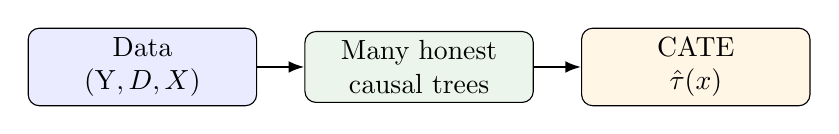
\begin{tikzpicture}[
  node distance=0.6cm,
  box/.style={draw, rounded corners, align=center, minimum width=2.9cm, minimum height=0.85cm},
  arrow/.style={-{Latex[length=2mm]}, thick}
]
  \node[box, fill=Blue!8]    (data)  {Data\\$(\mathrm{Y},D,X)$};
  \node[box, fill=Green!8,  right=of data]  (trees) {Many honest\\causal trees};
  \node[box, fill=Orange!10, right=of trees] (cate)  {CATE\\$\hat{\tau}(x)$};
  \draw[arrow] (data)  -- (trees);
  \draw[arrow] (trees) -- (cate);
\end{tikzpicture}
\end{center}
\vspace{0.1cm}
\begin{itemize}
  \item Each tree uses a \textbf{random subset} of observations and covariates; averaging trees removes noise and gives a stable $\hat{\tau}(x)$
\end{itemize}
\end{frame}

\begin{frame}{Running Example: Job Training}
\begin{itemize}
  \item Suppose a government offers a job training program.
  \vspace{0.2cm}
  \item Outcome $\mathrm{Y}_i$: earnings after the program.
  \vspace{0.2cm}
  \item Treatment $D_i$: whether worker $i$ received training.
  \vspace{0.2cm}
  \item Covariates $X_i$: age, education, race, marital status, previous earnings.
\end{itemize}

\vspace{0.35cm}
\begin{block}{Main policy question}
  Does the training program help everyone equally, or does it help some workers more than others?
\end{block}
\end{frame}

\begin{frame}{Why Heterogeneity Matters}
\begin{center}
\small
\begin{tabular}{lccc}
\toprule
Worker type & Control earnings & Training earnings & Effect \\
\midrule
Young, low education & \$8,000 & \$11,000 & \$3,000 \\
Older, high experience & \$18,000 & \$18,500 & \$500 \\
Disconnected worker & \$2,000 & \$6,000 & \$4,000 \\
\bottomrule
\end{tabular}
\end{center}

\vspace{0.3cm}
\begin{itemize}
  \item The average effect may look positive but modest.
  \item Policy decisions often require knowing \textbf{where} the effect is large.
  \item CATE helps answer: who should be prioritized if resources are limited?
\end{itemize}
\end{frame}

\begin{frame}{The Fundamental Causal Problem}
\begin{itemize}
  \item Each person has two potential outcomes:
  \[
    \mathrm{Y}^{1}_{i} \quad \text{if treated}, \qquad
    \mathrm{Y}^{0}_{i} \quad \text{if untreated}.
  \]
  \vspace{0.15cm}
  \item The individual treatment effect is $\tau_i=\mathrm{Y}^{1}_{i}-\mathrm{Y}^{0}_{i}$, but we only observe one outcome:
  \[
    \mathrm{Y}_i = D_i\mathrm{Y}^{1}_{i} + (1-D_i)\mathrm{Y}^{0}_{i}.
  \]
\end{itemize}

\vspace{0.2cm}
\begin{block}{Causal forest does not observe individual effects.}
  It estimates average effects for workers with \emph{similar} $X$ --- and it needs identification (RCT, DID, RDD, \ldots) to give these averages a causal interpretation.
\end{block}
\end{frame}

\begin{frame}{Traditional Approaches to Treatment Effect Heterogeneity}{}
\begin{itemize}
  \item Researchers have traditionally explored heterogeneity in two ways:
  \vspace{0.2cm}
  \begin{itemize}
    \item[1.] \textbf{Theory-based subgroup analysis}: guided by economic theory, split the sample by gender, age group, or education level and estimate the ATE in each subgroup
    \vspace{0.15cm}
    \item[2.] \textbf{Interaction terms in regression}:
    \[
      Y_i = \alpha + \beta D_i + \gamma X_i + \delta\,(D_i \times X_i) + \varepsilon_i
    \]
    the coefficient $\delta$ captures how the effect of $D_i$ varies linearly with $X_i$
  \end{itemize}
  \vspace{0.2cm}
  \item Both require the researcher to \textbf{pre-specify} which $X$ matters and assume a \textbf{linear, parametric} form for heterogeneity
\end{itemize}
\end{frame}

\begin{frame}{Causal Forest: A Data-Driven Approach}{}
\begin{itemize}
  \item Causal forest is \textbf{not} an identification strategy --- it does not solve the selection bias problem on its own
  \vspace{0.2cm}
  \item It is a flexible, \textbf{data-driven estimator} of CATE that can be paired with any identification strategy:
  \vspace{0.1cm}
  \begin{itemize}
    \item \textbf{RCT}: who benefits more from a randomized treatment?
    \vspace{0.1cm}
    \item \textbf{DID}: are treatment effects heterogeneous across groups?
    \vspace{0.1cm}
    \item \textbf{RDD}: who benefits most near the discontinuity threshold?
  \end{itemize}
  \vspace{0.2cm}
  \item Unlike subgroup analysis or interaction terms, causal forest \textbf{searches the data} for which characteristics drive heterogeneity --- without the researcher pre-specifying them
\end{itemize}
\end{frame}

\begin{frame}{How ATE and ATT Relate to CATE}
\begin{itemize}
  \item Once we know the CATE function $\tau(x)$, familiar estimands are just averages of it:
  \[
    \alpha_{\text{ATE}} = \mathrm{E}\!\left[\tau(X_i)\right], \qquad
    \alpha_{\text{ATT}} = \mathrm{E}\!\left[\tau(X_i)\mid D_i=1\right].
  \]
  \vspace{0.2cm}
  \item Causal forest therefore does not \emph{replace} ATE or ATT.
  \vspace{0.1cm}
  \begin{itemize}
    \item It estimates a richer object $\tau(x)$ first, and policy summaries such as ATE or ATT are recovered by averaging.
  \end{itemize}
  \vspace{0.2cm}
  \item This also means: if heterogeneity is small, $\tau(x) \approx \alpha_{\text{ATE}}$ for all $x$ --- causal forest collapses back to the usual ATE.
\end{itemize}
\end{frame}

%=============================================================
\title[]
{Decision Tree and Random Forest}

\subtitle{}
\author{}
\institute{}
\date{}

\begin{frame}{}
  \titlepage
\end{frame}

\section{Decision Tree and Random Forest}

\begin{frame}{Why We Need a Flexible Method}
\begin{itemize}
  \item One simple approach is to interact treatment with covariates:
  \[
    \mathrm{Y}_i
    =
    \delta+\alpha D_i+X_i\beta+(D_i\times X_i)\gamma+\epsilon_i.
  \]
  \vspace{0.2cm}
  \item This imposes a mostly linear structure.
  \vspace{0.2cm}
  \item But treatment effects may depend on nonlinear patterns:
  \begin{itemize}
    \item young \textit{and} low education,
    \item low previous earnings \textit{and} unmarried,
    \item thresholds such as age below 25 or earnings below zero.
  \end{itemize}
  \vspace{0.2cm}
  \item Causal forest searches for these patterns more flexibly.
\end{itemize}
\end{frame}

\begin{frame}{What Is a Decision Tree?}
\begin{itemize}
  \item A decision tree repeatedly asks yes/no questions about covariates $X_i$.
  \vspace{0.2cm}
  \item Each question splits the sample into smaller groups.
  \vspace{0.2cm}
  \item The final groups are called \textbf{leaves} or \textbf{terminal nodes}.
  \vspace{0.2cm}
  \item Within each leaf, the model uses a simple estimate:
  \[
    \hat{m}(\ell)=\frac{1}{N_\ell}\sum_{i:X_i\in \ell}\mathrm{Y}_i.
  \]
  \vspace{0.2cm}
  \item So a tree is a flexible way to create data-driven subgroups.
\end{itemize}
\end{frame}

\begin{frame}{Decision Tree: The Prediction Version}
\begin{center}
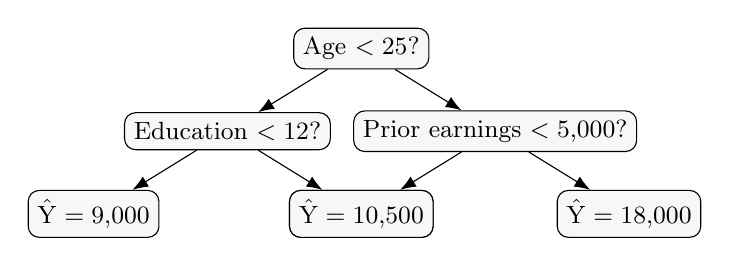
\begin{tikzpicture}[
  level distance=1.05cm,
  sibling distance=3.4cm,
  edge from parent/.style={draw,-{Latex[length=2mm]}},
  every node/.style={draw, rounded corners, align=center, font=\small, fill=gray!6}
]
\node {Age $<25$?}
  child {node {Education $<12$?}
    child {node {$\hat{\mathrm{Y}}=9{,}000$}}
    child {node {$\hat{\mathrm{Y}}=12{,}000$}}
  }
  child {node {Prior earnings $<5{,}000$?}
    child {node {$\hat{\mathrm{Y}}=10{,}500$}}
    child {node {$\hat{\mathrm{Y}}=18{,}000$}}
  };
\end{tikzpicture}
\end{center}

\vspace{0.25cm}
\begin{itemize}
  \item A tree partitions the covariate space into leaves.
  \item Prediction tree: each leaf predicts the average outcome $\hat{\mathrm{Y}}$.
  \item It is easy to interpret, but a single tree is unstable.
\end{itemize}
\end{frame}

\begin{frame}{Decision Tree: Partition of Covariate Space}
\begin{center}
\begin{tikzpicture}[x=0.12cm,y=0.12cm]
  \draw[->] (0,0) -- (60,0) node[right] {age};
  \draw[->] (0,0) -- (0,38) node[above] {education};
  \draw[thick, Blue] (25,0) -- (25,38);
  \draw[thick, Blue] (25,18) -- (60,18);
  \draw[thick, Blue] (0,24) -- (25,24);
  \node at (12,12) {Leaf 1};
  \node at (12,31) {Leaf 2};
  \node at (42,9) {Leaf 3};
  \node at (42,27) {Leaf 4};
  \node[below] at (25,0) {$25$};
  \node[left] at (0,24) {$12$};
  \node[left] at (0,18) {$10$};
\end{tikzpicture}
\end{center}

\vspace{0.2cm}
\begin{itemize}
  \item A tree divides the $X$-space into rectangular regions.
  \item People in the same leaf receive the same prediction.
  \item Deeper trees create smaller groups and more flexible predictions.
\end{itemize}
\end{frame}

\begin{frame}{How a Prediction Tree Chooses Splits}
\begin{itemize}
  \item A prediction tree chooses the split that best predicts $\mathrm{Y}_i$.
  \vspace{0.2cm}
  \item For each candidate split, compare prediction errors:
  \[
    \sum_{i\in R_1}\left(\mathrm{Y}_i-\bar{Y}_{R_1}\right)^2
    +
    \sum_{i\in R_2}\left(\mathrm{Y}_i-\bar{Y}_{R_2}\right)^2.
  \]
  \vspace{0.2cm}
  \item The tree chooses the split with the smallest residual sum of squares.
  \vspace{0.2cm}
  \item Intuition: put people with similar outcomes into the same leaf.
\end{itemize}
\end{frame}

\begin{frame}{Why a Single Tree Is Not Enough}
\begin{itemize}
  \item A single decision tree is easy to interpret.
  \vspace{0.2cm}
  \item But it has \textbf{high variance}:
  \vspace{0.1cm}
  \begin{itemize}
    \item small changes in the data can change the first split,
    \item changing the first split changes all later splits,
    \item predictions can be unstable.
  \end{itemize}
  \vspace{0.25cm}
  \item This matters even more for causal inference because treatment-effect estimates are noisier than outcome means.
\end{itemize}

\vspace{0.2cm}
\begin{block}{Core problem}
One tree is too dependent on one particular sample.
\end{block}
\end{frame}

\begin{frame}{Random Forest: Stabilize Trees by Averaging}
\begin{itemize}
  \item A random forest grows many trees on different random subsamples.
  \vspace{0.2cm}
  \item Each tree is noisy, but the average is more stable:
  \[
    \hat{m}(x)=\frac{1}{B}\sum_{b=1}^B \hat{m}_b(x).
  \]
  \vspace{0.2cm}
  \item Prediction random forest estimates:
  \[
    m(x)=\mathrm{E}\!\left[\mathrm{Y}_i\mid X_i=x\right].
  \]
  \vspace{0.2cm}
  \item Causal forest keeps the forest idea, but changes the target from outcome prediction to treatment effect estimation.
\end{itemize}
\end{frame}

\begin{frame}{Random Forest: Two Sources of Diversity}
\begin{itemize}
  \item A random forest makes trees different from one another.
  \vspace{0.25cm}
  \item \textbf{Subsampling:}
  \begin{itemize}
    \item each tree sees a different random subset of observations,
    \item each tree learns a slightly different pattern.
  \end{itemize}
  \vspace{0.25cm}
  \item \textbf{Random split variables:}
  \begin{itemize}
    \item at each split, the tree considers only a random subset of covariates,
    \item this prevents all trees from looking too similar.
  \end{itemize}
  \vspace{0.25cm}
  \item Averaging works best when trees are individually useful but not identical.
\end{itemize}
\end{frame}

\begin{frame}{Bridge to Causal Forest}
\begin{center}
\small
\begin{tabular}{lll}
\toprule
Step & Prediction forest & Causal forest \\
\midrule
Tree creates leaves & similar outcomes & similar treatment effects \\
Leaf estimate & $\bar{Y}_{\ell}$ & $\bar{Y}^{1}_{\ell}-\bar{Y}^{0}_{\ell}$ \\
Forest average & $\hat{m}(x)$ & $\hat{\tau}(x)$ \\
Main question & what outcome is likely? & who benefits more? \\
\bottomrule
\end{tabular}
\end{center}

\vspace{0.3cm}
\begin{block}{The key transition}
Causal forest keeps the tree-and-forest machinery, but replaces prediction of $\mathrm{Y}$ with estimation of $\tau(x)$.
\end{block}
\end{frame}

%=============================================================
\title[]
{Causal Tree}

\subtitle{}
\author{}
\institute{}
\date{}

\begin{frame}{}
  \titlepage
\end{frame}

\section{Causal Tree}

\begin{frame}{From Prediction Tree to Causal Tree}
\begin{center}
\small
\begin{tabular}{lll}
\toprule
 & Prediction tree & Causal tree \\
\midrule
Target & outcome $\mathrm{Y}$ & treatment effect $\tau(x)$ \\
Split tries to find & different levels of $\mathrm{Y}$ & different effects of $D$ \\
Leaf estimate & $\bar{Y}$ & $\bar{Y}^{1}_{\ell}-\bar{Y}^{0}_{\ell}$ \\
Question & who has high earnings? & who gains more from training? \\
\bottomrule
\end{tabular}
\end{center}

\vspace{0.35cm}
\begin{block}{Key change}
Instead of grouping people with similar outcomes, a causal tree groups people with similar treatment effects.
\end{block}
\end{frame}

\begin{frame}{Causal Tree: Leaf-Level Intuition}
\begin{center}
\small
\begin{tabular}{lccc}
\toprule
Leaf & Treated mean & Control mean & Estimated effect \\
\midrule
Young, low education & \$11,000 & \$8,000 & \$3,000 \\
Older, high experience & \$18,500 & \$18,000 & \$500 \\
\bottomrule
\end{tabular}
\end{center}

\vspace{0.3cm}
\begin{itemize}
  \item Within each leaf, compare treated and control workers.
  \vspace{0.2cm}
  \item The leaf estimate is a local average treatment effect:
  \[
    \hat{\tau}(\ell)=\bar{Y}^{1}_{\ell}-\bar{Y}^{0}_{\ell}.
  \]
  \vspace{0.2cm}
  \item A new worker receives the estimate from the leaf containing their $X_i$.
\end{itemize}
\end{frame}

\begin{frame}{Causal Tree: Finding a Split}
\begin{enumerate}
  \item For each variable $X^j$ and candidate split point $s$, create two regions:
  \[
    R_1(j,s)=\{i:X_i^j<s\},
    \qquad
    R_2(j,s)=\{i:X_i^j\geq s\}.
  \]
  \vspace{0.15cm}
  \item Estimate the treatment effect in each region:
  \[
    \hat{\tau}(R)=\bar{Y}^{1}_{R}-\bar{Y}^{0}_{R}.
  \]
  \vspace{0.15cm}
  \item Choose splits that reveal treatment-effect heterogeneity:
  \[
    \Delta(j,s)
    =
    \left|\hat{\tau}(R_1)-\hat{\tau}(R_2)\right|.
  \]
\end{enumerate}

\vspace{0.1cm}
\begin{center}
\textbf{A causal tree looks for different effects, not just different outcomes.}
\end{center}
\end{frame}

\begin{frame}{Causal Tree: A Small Split Example}
\begin{center}
\small
\begin{tabular}{lccc}
\toprule
Candidate split & $\hat{\tau}(R_1)$ & $\hat{\tau}(R_2)$ & $\Delta$ \\
\midrule
Age $<30$ & \$3,000 & \$600 & \textbf{\$2,400} \\
Education $<12$ & \$2,100 & \$1,400 & \$700 \\
Prior earnings $<5{,}000$ & \$2,600 & \$1,000 & \$1,600 \\
\bottomrule
\end{tabular}
\end{center}

\vspace{0.3cm}
\begin{itemize}
  \item In this toy example, the tree would first split on age.
  \vspace{0.2cm}
  \item The point is not that age is always important.
  \vspace{0.2cm}
  \item The tree selects the variable and threshold that best separate high-effect and low-effect groups in the data.
\end{itemize}
\end{frame}

\begin{frame}{The Main Problem: Double Dipping}
\begin{itemize}
  \item If the same data are used to:
  \begin{enumerate}
    \item choose the split, and
    \item estimate the treatment effect in the leaves,
  \end{enumerate}
  the tree can overfit random noise.
  \vspace{0.3cm}
  \item A split may look good simply because it got lucky in this sample.
  \vspace{0.3cm}
  \item Then leaf treatment effects are biased upward in magnitude.
\end{itemize}

\vspace{0.25cm}
\begin{block}{Teaching intuition}
The tree used the data to search over many possible splits, so the chosen split may look too good.
\end{block}
\end{frame}

\begin{frame}{Honest Estimation}
\begin{center}
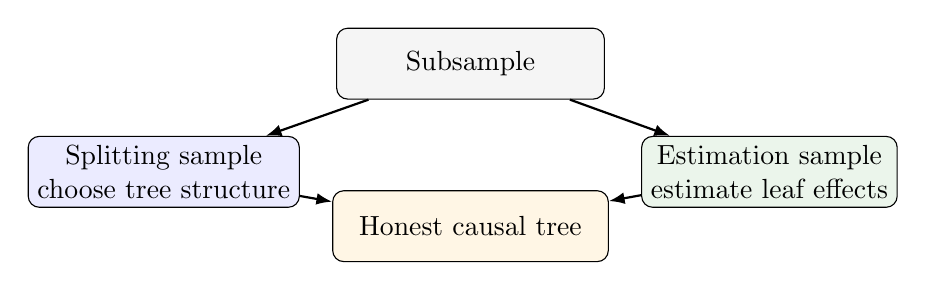
\begin{tikzpicture}[
  box/.style={draw, rounded corners, align=center, minimum height=0.9cm},
  arrow/.style={-{Latex[length=2mm]}, thick},
  node distance=0.65cm
]
\node[box, fill=gray!8, minimum width=3.4cm] (sample) {Subsample};
\node[box, fill=Blue!8, below left=of sample, minimum width=3.2cm] (split) {Splitting sample\\choose tree structure};
\node[box, fill=Green!8, below right=of sample, minimum width=3.2cm] (estimate) {Estimation sample\\estimate leaf effects};
\node[box, fill=Orange!10, below=1.15cm of sample, minimum width=3.5cm] (tree) {Honest causal tree};
\draw[arrow] (sample) -- (split);
\draw[arrow] (sample) -- (estimate);
\draw[arrow] (split) -- (tree);
\draw[arrow] (estimate) -- (tree);
\end{tikzpicture}
\end{center}

\vspace{0.2cm}
\begin{itemize}
  \item One part of the data decides where to split.
  \item A separate part estimates treatment effects in the final leaves.
  \item This reduces overfitting and supports valid inference.
\end{itemize}
\end{frame}

%=============================================================
\title[]
{Causal Forest}

\subtitle{}
\author{}
\institute{}
\date{}

\begin{frame}{}
  \titlepage
\end{frame}

\section{Causal Forest}

\begin{frame}{Causal Forest Algorithm}
\begin{enumerate}
  \item Draw a random subsample of observations.
  \vspace{0.15cm}
  \item Split the subsample into two parts:
  \begin{itemize}
    \item one for choosing splits,
    \item one for estimating treatment effects.
  \end{itemize}
  \vspace{0.15cm}
  \item Grow an honest causal tree.
  \vspace{0.15cm}
  \item Repeat many times, for example $B=2{,}000$ trees.
  \vspace{0.15cm}
  \item For each observation, average the estimates from all trees:
  \[
    \hat{\tau}(x_i)=\frac{1}{B}\sum_{b=1}^B \hat{\tau}_b(x_i).
  \]
\end{enumerate}
\end{frame}

\begin{frame}{Causal Forest as Adaptive Weighting}
\begin{itemize}
  \item Another useful way to view causal forest:
  \vspace{0.1cm}
  \begin{itemize}
    \item for a target worker with characteristics $x$,
    \item the forest finds other workers who often fall in the same leaves as $x$,
    \item those workers receive larger weights in estimating $\tau(x)$.
  \end{itemize}
  \vspace{0.25cm}
  \item Conceptually:
  \[
    \hat{\tau}(x)
    \approx
    \sum_{i:D_i=1} a_i(x)\mathrm{Y}_i
    -
    \sum_{i:D_i=0} a_i(x)\mathrm{Y}_i,
  \]
  where $a_i(x)$ is larger when observation $i$ is similar to $x$ according to the forest.
  \vspace{0.25cm}
  \item This is why causal forest is like a flexible matching method plus valid forest-based inference.
\end{itemize}
\end{frame}

\begin{frame}{Why Averaging Helps}
\begin{itemize}
  \item A single causal tree is interpretable but noisy.
  \vspace{0.2cm}
  \item Different subsamples produce different trees.
  \vspace{0.2cm}
  \item Averaging many trees reduces variance:
  \[
    \hat{\tau}_b(x)=\tau(x)+\varepsilon_b,
    \qquad
    \frac{1}{B}\sum_{b=1}^B \hat{\tau}_b(x)
    =
    \tau(x)+\frac{1}{B}\sum_{b=1}^B \varepsilon_b.
  \]
  \vspace{0.2cm}
  \item If the tree-specific errors partly cancel out, the forest estimate is more stable.
\end{itemize}
\end{frame}

\begin{frame}{Random Forest vs. Causal Forest}
\begin{center}
\small
\begin{tabular}{lll}
\toprule
 & Random forest & Causal forest \\
\midrule
Main goal & predict outcome & estimate treatment effect \\
Input & $(\mathrm{Y},X)$ & $(\mathrm{Y},D,X)$ \\
Object & $\hat{m}(x)$ & $\hat{\tau}(x)$ \\
Split criterion & reduce prediction error & find effect heterogeneity \\
Leaf value & mean outcome & treated-control difference \\
Honesty & usually no & yes \\
\bottomrule
\end{tabular}
\end{center}

\vspace{0.3cm}
\begin{block}{Do not confuse these two}
A causal forest is not just a random forest with treatment added as another predictor.
\end{block}
\end{frame}

\begin{frame}{Statistical Properties: What to Know}
\begin{itemize}
  \item Honest causal forest is designed for both estimation and inference.
  \vspace{0.2cm}
  \item Under regularity conditions:
  \[
    \hat{\tau}(x)\xrightarrow{p}\tau(x)
    \qquad \text{as } N\to\infty.
  \]
  \vspace{0.2cm}
  \item The \texttt{grf} package reports standard errors for ATE and related summaries.
  \vspace{0.2cm}
  \item For teaching purposes, the key idea is:
  \vspace{0.1cm}
  \begin{itemize}
    \item honesty controls adaptive bias,
    \item averaging many trees reduces variance,
    \item valid causal interpretation still comes from the research design.
  \end{itemize}
\end{itemize}
\end{frame}

\begin{frame}{What Does $\hat{\tau}(x_i)$ Mean?}
\begin{itemize}
  \item $\hat{\tau}(x_i)$ is not the true individual treatment effect.
  \vspace{0.2cm}
  \item It estimates the average treatment effect for people similar to worker $i$.
  \vspace{0.2cm}
  \item Similarity is learned by the forest from covariates $X$.
  \vspace{0.2cm}
  \item Interpretation in the job training example:
  \[
    \hat{\tau}(x_i)=2{,}000
  \]
  means workers with similar characteristics to worker $i$ are estimated to gain about \$2,000 from training.
\end{itemize}
\end{frame}

\begin{frame}{What Causal Forest Gives Us}
\begin{itemize}
  \item \textbf{ATE}: $\hat{\alpha}_{\text{ATE}}$ in the target sample.
  \vspace{0.2cm}
  \item \textbf{ATT}: $\hat{\alpha}_{\text{ATT}}$ for treated observations.
  \vspace{0.2cm}
  \item \textbf{CATE estimates}: one $\hat{\tau}(x_i)$ for each observation.
  \vspace{0.2cm}
  \item \textbf{CATE distribution}: whether effects are concentrated or very different across people.
  \vspace{0.2cm}
  \item \textbf{Best linear projection}: which covariates are associated with larger effects.
  \vspace{0.2cm}
  \item \textbf{Variable importance}: which variables are often used to split treatment-effect heterogeneity.
\end{itemize}
\end{frame}

\begin{frame}{How to Read the CATE Distribution}
\begin{center}
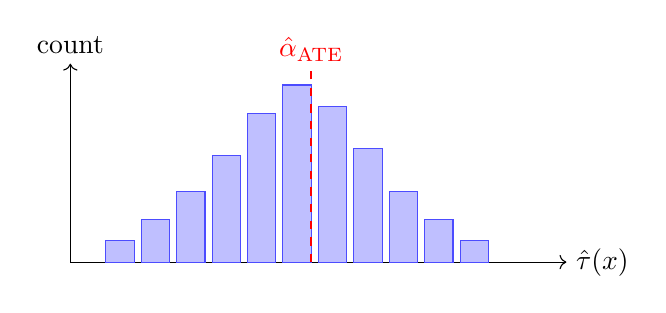
\begin{tikzpicture}[x=0.09cm,y=0.09cm]
  \draw[->] (0,0) -- (70,0) node[right] {$\hat{\tau}(x)$};
  \draw[->] (0,0) -- (0,28) node[above] {count};
  \foreach \x/\h in {5/3,10/6,15/10,20/15,25/21,30/25,35/22,40/16,45/10,50/6,55/3}
    \draw[fill=Blue!25, draw=Blue!70] (\x,0) rectangle ++(4,\h);
  \draw[red, thick, dashed] (34,0) -- (34,27);
  \node[red, above] at (34,27) {$\hat{\alpha}_{\text{ATE}}$};
\end{tikzpicture}
\end{center}

\vspace{0.2cm}
\begin{itemize}
  \item A wide distribution suggests substantial heterogeneity.
  \item A narrow distribution suggests the treatment effect is similar for most people.
  \item The average can hide both winners and non-responders.
\end{itemize}
\end{frame}

\begin{frame}{BLP: A Simple Summary of Heterogeneity}
\begin{itemize}
  \item CATE estimates can be hard to summarize one by one.
  \vspace{0.2cm}
  \item Best linear projection asks:
  \[
    \hat{\tau}(x_i)
    =
    \beta_0+\beta_1\,\text{age}_i+\beta_2\,\text{educ}_i+\beta_3\,\text{re74}_i+\cdots+\varepsilon_i.
  \]
  \vspace{0.2cm}
  \item Example interpretations:
  \begin{itemize}
    \item $\hat{\beta}_1<0$: older workers tend to benefit less.
    \item $\hat{\beta}_3<0$: workers with higher previous earnings tend to benefit less.
  \end{itemize}
  \vspace{0.2cm}
  \item BLP is descriptive: it summarizes the forest's estimated heterogeneity.
\end{itemize}
\end{frame}

\begin{frame}{Variable Importance}
\begin{itemize}
  \item Variable importance asks which variables the forest often uses to split.
  \vspace{0.2cm}
  \item A high value means the variable is useful for finding groups with different treatment effects.
  \vspace{0.2cm}
  \item It can detect nonlinearities and interactions.
  \vspace{0.2cm}
  \item But it does not tell the sign of the relationship.
\end{itemize}

\vspace{0.3cm}
\begin{center}
\small
\begin{tabular}{ll}
\toprule
BLP & direction and standard errors \\
Variable importance & which variables help split the forest \\
\bottomrule
\end{tabular}
\end{center}
\end{frame}

\begin{frame}{Practical Warnings}
\begin{itemize}
  \item Do not interpret CATE estimates causally without a credible identification strategy.
  \vspace{0.2cm}
  \item Do not overinterpret one person's estimate; think in terms of similar groups.
  \vspace{0.2cm}
  \item Check overlap: for each region of $X$, we need both treated and control observations.
  \vspace{0.2cm}
  \item Use forests for exploration and targeting, then report simple summaries carefully.
  \vspace{0.2cm}
  \item In small samples, heterogeneity estimates can be noisy.
\end{itemize}
\end{frame}

%=============================================================
\title[]
{R Example: Job Training Program}

\subtitle{}
\author{}
\institute{}
\date{}

\begin{frame}{}
  \titlepage
\end{frame}

\section{R Example}

\begin{frame}{LaLonde Job Training Data}{R Implementation}
\begin{itemize}
  \item Classic job training dataset from LaLonde (1986).
  \vspace{0.2cm}
  \item Treatment $D_i$: participation in the training program.
  \vspace{0.2cm}
  \item Outcome $\mathrm{Y}_i$: earnings in 1978.
  \vspace{0.2cm}
  \item Covariates $X_i$: age, education, race, marital status, no degree, earnings in 1974 and 1975.
  \vspace{0.2cm}
  \item Main question: which workers gain more from training?
  \vspace{0.2cm}
  \item R workflow:
  \begin{itemize}
    \item Step 1: install packages and load data
    \item Step 2: prepare $\mathrm{Y}_i$, $D_i$, and $X_i$
    \item Step 3: estimate causal forest
    \item Step 4: report ATE/ATT and CATE heterogeneity
  \end{itemize}
\end{itemize}
\end{frame}

\begin{frame}[fragile]{Step 1: Package Installation and Data Loading}
\begin{itemize}
  \item Install and load required R packages:
\begin{lstlisting}[style=r-style]
install.packages(c("grf", "Matching", "ggplot2"))

library(grf)
library(Matching)
library(ggplot2)
\end{lstlisting}
  \vspace{0.1cm}
  \item Load the LaLonde data:
\begin{lstlisting}[style=r-style]
data(lalonde)
summary(lalonde)
\end{lstlisting}
  \vspace{0.1cm}
  \item \texttt{grf}: generalized random forests.
  \item \texttt{Matching}: includes the LaLonde dataset.
  \item \texttt{ggplot2}: visualization.
\end{itemize}
\end{frame}

\begin{frame}[fragile]{Step 2: Data Preparation}
\begin{itemize}
  \item Define outcome $\mathrm{Y}_i$, treatment $D_i$, and covariates $X_i$:
\begin{lstlisting}[style=r-style]
Y <- lalonde$re78
D <- lalonde$treat
X <- lalonde[, c("age", "educ", "black", "hisp",
                 "married", "nodegree", "re74", "re75")]
X <- as.matrix(X)
\end{lstlisting}
  \vspace{0.1cm}
  \item \texttt{Y}: observed outcome $\mathrm{Y}_i$.
  \item \texttt{D}: treatment indicator $D_i$.
  \item \texttt{X}: pre-treatment covariates.
  \item All variables in \texttt{X} should be measured before treatment.
\end{itemize}
\end{frame}

\begin{frame}[fragile]{Step 3: Causal Forest Estimation}
\begin{itemize}
  \item Estimate the causal forest:
\begin{lstlisting}[style=r-style]
set.seed(2026)

cf <- causal_forest(
  X = X,
  Y = Y,
  W = D,
  num.trees = 2000
)
\end{lstlisting}
  \vspace{0.1cm}
  \item \texttt{causal\_forest()} estimates heterogeneous treatment effects.
  \item \texttt{W = D}: \texttt{grf} names the treatment argument \texttt{W}, but our course notation is $D_i$.
  \item \texttt{num.trees = 2000}: more trees usually produce more stable estimates.
  \item The package handles honesty and forest averaging internally.
\end{itemize}
\end{frame}

\begin{frame}[fragile]{Step 4: Estimate ATE and ATT}
\begin{itemize}
  \item Report the average treatment effect and the effect on the treated:
\begin{lstlisting}[style=r-style]
ate <- average_treatment_effect(cf, target.sample = "all")
att <- average_treatment_effect(cf, target.sample = "treated")

ate
att
\end{lstlisting}
  \vspace{0.1cm}
  \item Returns the estimated average treatment effect and standard error.
  \item \texttt{target.sample = "all"} estimates $\alpha_{\text{ATE}}$.
  \item \texttt{target.sample = "treated"} estimates $\alpha_{\text{ATT}}$.
  \item These connect the new method back to the earlier course estimands.
\end{itemize}
\end{frame}

\begin{frame}{What ATE and ATT Mean Here}
\begin{itemize}
  \item The forest first estimates individual CATEs $\hat{\tau}(x_i)$.
  \vspace{0.2cm}
  \item Then it averages them over different target samples:
  \[
    \hat{\alpha}_{\text{ATE}}
    \approx
    \frac{1}{N}\sum_{i=1}^N\hat{\tau}(x_i),
    \qquad
    \hat{\alpha}_{\text{ATT}}
    \approx
    \frac{1}{N_1}\sum_{i:D_i=1}\hat{\tau}(x_i).
  \]
  \vspace{0.2cm}
  \item In practice, \texttt{grf} uses forest weights and influence-function adjustments, so the package estimate is the preferred reported number.
\end{itemize}
\end{frame}

\begin{frame}[fragile]{Step 5: Get CATE Estimates}
\begin{itemize}
  \item Predict the CATE for each observation:
\begin{lstlisting}[style=r-style]
tau_hat <- predict(cf)$predictions

summary(tau_hat)
\end{lstlisting}
  \vspace{0.1cm}
  \item \texttt{tau\_hat} contains one estimated CATE for each observation.
  \item Interpretation: $\hat{\tau}(x_i)$ is the estimated training effect for workers similar to $i$.
  \item Use the summary to see whether effects look similar or very dispersed.
\end{itemize}
\end{frame}

\begin{frame}[fragile]{Step 6: Plot CATE Distribution}
\begin{itemize}
  \item Plot the distribution of estimated CATEs:
\begin{lstlisting}[style=r-style]
cate_df <- data.frame(tau_hat = tau_hat)

ggplot(cate_df, aes(x = tau_hat)) +
  geom_histogram(bins = 30, fill = "steelblue",
                 color = "white") +
  geom_vline(xintercept = mean(tau_hat),
             color = "red", linetype = "dashed") +
  labs(x = "Estimated treatment effect",
       y = "Count")
\end{lstlisting}
  \vspace{0.1cm}
  \item The red line is the average of the estimated CATEs.
  \item The spread shows the amount of estimated heterogeneity.
\end{itemize}
\end{frame}

\begin{frame}[fragile]{Step 7: Summarize Heterogeneity}
\begin{itemize}
  \item Use BLP and variable importance:
\begin{lstlisting}[style=r-style]
# Best linear projection
blp <- best_linear_projection(cf, X)
blp

# Variable importance
vi <- variable_importance(cf)
names(vi) <- colnames(X)
sort(vi, decreasing = TRUE)
\end{lstlisting}
  \vspace{0.1cm}
  \item BLP helps interpret which covariates are associated with larger effects.
  \item Variable importance helps identify which covariates are useful for splitting.
  \item Read them as summaries of heterogeneity, not as a replacement for the research design.
\end{itemize}
\end{frame}

\begin{frame}[fragile]{Step 8: Export for Stata Post-Analysis}
\begin{itemize}
  \item Export CATE estimates for familiar post-analysis:
\begin{lstlisting}[style=r-style]
results <- data.frame(
  id      = 1:nrow(X),
  tau_hat = tau_hat,
  age     = lalonde$age,
  educ    = lalonde$educ,
  D       = lalonde$treat
)

write.csv(results, "cate_results.csv",
          row.names = FALSE)
\end{lstlisting}
  \vspace{0.1cm}
  \item Estimate the forest in R.
  \item Export CATE estimates for familiar summary tables and plots elsewhere.
\end{itemize}
\end{frame}

%=============================================================
\title[]
{Labor Economics Application}

\subtitle{}
\author{}
\institute{}
\date{}

\begin{frame}{}
  \titlepage
\end{frame}

\section{Application and Wrap-Up}

\begin{frame}{Labor Economics Applications}
\begin{itemize}
  \item Active labor market programs: who benefits from job search assistance?
  \vspace{0.2cm}
  \item Youth employment programs: which youth benefit most?
  \vspace{0.2cm}
  \item Education policy: do returns differ by background or local labor market?
  \vspace{0.2cm}
  \item Minimum wage: do effects differ by worker skill, firm size, or region?
  \vspace{0.2cm}
  \item Parental leave: do effects differ by previous earnings or occupation?
\end{itemize}
\end{frame}

\begin{frame}{What Students Should Remember}
\begin{enumerate}
  \item Earlier lectures focused on $\alpha_{\text{ATE}}$ and $\alpha_{\text{ATT}}$.
  \vspace{0.2cm}
  \item CATE asks how effects vary with $X_i$:
  \[
    \tau(x)=\mathrm{E}\!\left[\mathrm{Y}^{1}_{i}-\mathrm{Y}^{0}_{i}\mid X_i=x\right].
  \]
  \vspace{0.2cm}
  \item A decision tree creates data-driven subgroups; a random forest stabilizes trees by averaging.
  \vspace{0.2cm}
  \item A causal tree changes the target from outcome prediction to treatment-effect heterogeneity.
  \vspace{0.2cm}
  \item Honesty separates split selection from effect estimation.
  \vspace{0.2cm}
  \item A causal forest averages many honest causal trees to stabilize $\hat{\tau}(x)$.
\end{enumerate}
\end{frame}

\begin{frame}{Checklist for Using Causal Forest}
\begin{enumerate}
  \item Define the outcome $\mathrm{Y}_i$, treatment $D_i$, and pre-treatment covariates $X_i$.
  \vspace{0.15cm}
  \item Explain the causal identification assumption.
  \vspace{0.15cm}
  \item Check overlap: both treated and control observations should exist across relevant $X_i$ regions.
  \vspace{0.15cm}
  \item Estimate the forest and report $\hat{\alpha}_{\text{ATE}}$ or $\hat{\alpha}_{\text{ATT}}$.
  \vspace{0.15cm}
  \item Use CATE distribution, BLP, and variable importance to describe heterogeneity.
\end{enumerate}
\end{frame}

%=============================================================
\title[]
{Recommended Resources}

\subtitle{}
\author{}
\institute{}
\date{}

\begin{frame}{}
  \titlepage
\end{frame}

\begin{frame}{Recommended Resources}
\begin{itemize}
  \item Wager and Athey (2018), ``Estimation and Inference of Heterogeneous Treatment Effects using Random Forests.''
  \vspace{0.2cm}
  \item Athey, Tibshirani, and Wager (2019), ``Generalized Random Forests.''
  \vspace{0.2cm}
  \item \texttt{grf} documentation:
  \begin{center}
    \url{https://grf-labs.github.io/grf/}
  \end{center}
  \vspace{0.2cm}
  \item Athey and Imbens (2019), ``Machine Learning Methods That Economists Should Know About.''
\end{itemize}
\end{frame}

\begin{frame}{Final Takeaway}
\begin{center}
\large
Causal forest helps us move from

\vspace{0.25cm}
\textbf{``Does the policy work on average?''}

\vspace{0.25cm}
to

\vspace{0.25cm}
\textbf{``For whom does the policy work best?''}
\end{center}

\vspace{0.3cm}
\begin{block}{But}
The forest estimates heterogeneity. The research design still provides the causal credibility.
\end{block}
\end{frame}

\end{document}
